
%(BEGIN_QUESTION)
% Copyright 2010, Tony R. Kuphaldt, released under the Creative Commons Attribution License (v 1.0)
% This means you may do almost anything with this work of mine, so long as you give me proper credit

This analog electronic controller circuit has a problem.  The output signal is saturated over 100\% no matter what signals are input to the PV terminal, and no matter where the SP is adjusted to:

$$\includegraphics[width=15.5cm]{i01416x01.eps}$$

With the PV input signal at +3.00 volts and the setpoint signal at +2.58 volts, a technician measures $-0.42$ volts DC at test point TP5.  Identify the likelihood of each specified fault for this circuit.  Consider each fault one at a time (i.e. no coincidental faults), determining whether or not each fault could independently account for {\it all} measurements and symptoms in this circuit.

% No blank lines allowed between lines of an \halign structure!
% I use comments (%) instead, so that TeX doesn't choke.

$$\vbox{\offinterlineskip
\halign{\strut
\vrule \quad\hfil # \ \hfil & 
\vrule \quad\hfil # \ \hfil & 
\vrule \quad\hfil # \ \hfil \vrule \cr
\noalign{\hrule}
%
% First row
{\bf Fault} & {\bf Possible} & {\bf Impossible} \cr
%
\noalign{\hrule}
%
% Another row
Opamp $U_1$ output failed to low rail &  &  \cr
%
\noalign{\hrule}
%
% Another row
Opamp $U_4$ output failed to high rail &  &  \cr
%
\noalign{\hrule}
%
% Another row
Opamp $U_5$ output failed to low rail &  &  \cr
%
\noalign{\hrule}
%
% Another row
$R_1$ connection to ground failed open &  &  \cr
%
\noalign{\hrule}
%
% Another row
$R_3$ connection to +V failed open &  &  \cr
%
\noalign{\hrule}
%
% Another row
Resistor $R_8$ failed open &  &  \cr
%
\noalign{\hrule}
%
% Another row
Resistor $R_9$ failed open &  &  \cr
%
\noalign{\hrule}
%
% Another row
Resistor $R_{10}$ failed open &  &  \cr
%
\noalign{\hrule}
%
% Another row
Resistor $R_{11}$ failed open &  &  \cr
%
\noalign{\hrule}
} % End of \halign 
}$$ % End of \vbox

Finally, identify the {\it next} diagnostic test or measurement you would make on this system.  Explain how the result(s) of this next test or measurement help further identify the location and/or nature of the fault.

\vskip 20pt \vbox{\hrule \hbox{\strut \vrule{} {\bf Suggestions for Socratic discussion} \vrule} \hrule}

\begin{itemize}
\item{} Calculate the appropriate position for potentiometer $R_1$ in order to set the bias value of this controller to 50\%.
\end{itemize}

\underbar{file i01416}
%(END_QUESTION)





%(BEGIN_ANSWER)

% No blank lines allowed between lines of an \halign structure!
% I use comments (%) instead, so that TeX doesn't choke.

$$\vbox{\offinterlineskip
\halign{\strut
\vrule \quad\hfil # \ \hfil & 
\vrule \quad\hfil # \ \hfil & 
\vrule \quad\hfil # \ \hfil \vrule \cr
\noalign{\hrule}
%
% First row
{\bf Fault} & {\bf Possible} & {\bf Impossible} \cr
%
\noalign{\hrule}
%
% Another row
Opamp $U_1$ output failed to low rail &  & $\surd$ \cr
%
\noalign{\hrule}
%
% Another row
Opamp $U_4$ output failed to high rail &  & $\surd$ \cr
%
\noalign{\hrule}
%
% Another row
Opamp $U_5$ output failed to low rail & $\surd$ &  \cr
%
\noalign{\hrule}
%
% Another row
$R_1$ connection to ground failed open & $\surd$ &  \cr
%
\noalign{\hrule}
%
% Another row
$R_3$ connection to +V failed open &  & $\surd$ \cr
%
\noalign{\hrule}
%
% Another row
Resistor $R_8$ failed open &  & $\surd$ \cr
%
\noalign{\hrule}
%
% Another row
Resistor $R_9$ failed open & ? &  \cr
%
\noalign{\hrule}
%
% Another row
Resistor $R_{10}$ failed open & ? &  \cr
%
\noalign{\hrule}
%
% Another row
Resistor $R_{11}$ failed open &  & $\surd$ \cr
%
\noalign{\hrule}
} % End of \halign 
}$$ % End of \vbox

$R_1$ connection to ground failed open is possible because that potentiometer connects to the negative power supply rail (-V) and thus an open ground would make the bias signal go fully negative, driving the controller's output fully positive.

\vskip 10pt

An open $R_9$ or open $R_{10}$ makes sense only for certain (large) values of bias, if the output never deviates from full saturation {\it no matter what values are input to PV or SP}.

%(END_ANSWER)





%(BEGIN_NOTES)

A good ``next test'' would be to measure the output of the next opamp stage (TP7) to see if the signal still ``makes sense'' there as well, since the signal we measured at TP5 was good (the difference between PV and SP).





\filbreak \vskip 20pt \vbox{\hrule \hbox{\strut \vrule{} {\bf Virtual Troubleshooting} \vrule} \hrule}

\noindent
{\bf Predicting the effect of a given fault:} present each of the following faults to the students, one at a time, having them comment on all the effects each fault would produce.

\begin{itemize}
\item{} Resistor $R_5$ fails open
\item{} Resistor $R_6$ fails open
\item{} Resistor $R_7$ fails open
\item{} Resistor $R_8$ fails open
\item{} Resistor $R_9$ fails open
\item{} Resistor $R_{10}$ fails open
\item{} Resistor $R_{11}$ fails open
\item{} TP5 shorts to ground 
\item{} TP6 shorts to ground 
\item{} TP7 shorts to ground 
\item{} TP8 shorts to ground 
\item{} Null voltmeter fails open
\item{} Opamp $U_1$ fails with low output
\item{} Opamp $U_3$ fails with high output
\item{} Opamp $U_4$ fails with low output
\item{} Opamp $U_5$ fails with high output
\end{itemize}


\vskip 10pt


\noindent
{\bf Identifying possible/impossible faults:} present symptoms to the students and then have them determine whether or not a series of suggested faults could account for all the symptoms, explaining {\it why} or {\it why not} for each proposed fault:

\begin{itemize}
\item{} Symptom: {\it }
\item{} 
\item{} 
\item{} 
\end{itemize}


\vskip 10pt


\noindent
{\bf Determining the utility of given diagnostic tests:} present symptoms to the students and then propose the following diagnostic tests one by one.  Students rate the value of each test, determining whether or not it would give useful information (i.e. tell us something we don't already know).  Students determine what different results for each test would indicate about the fault, if anything:

\begin{itemize}
\item{} Symptom: {\it }
\item{}  -- {\bf Yes/No}
\item{}  -- {\bf Yes/No}
\end{itemize}


\vskip 10pt


\noindent
{\bf Diagnosing a fault based on given symptoms:} imagine the ??? fails ??? in this system (don't reveal the fault to students!).  Present the operator's observation(s) to the students, have them consider possible faults and diagnostic strategies, and then tell them the results of tests they propose based on the following symptoms, until they have properly identified the nature and location of the fault:

\begin{itemize}
\item{} {\it }
\item{} 
\item{} 
\end{itemize}
%INDEX% Control, proportional: analog electronic controller

%(END_NOTES)

